\subsection{Damage and ground-motion intensity map selection problem}

\begin{figure}
\centering
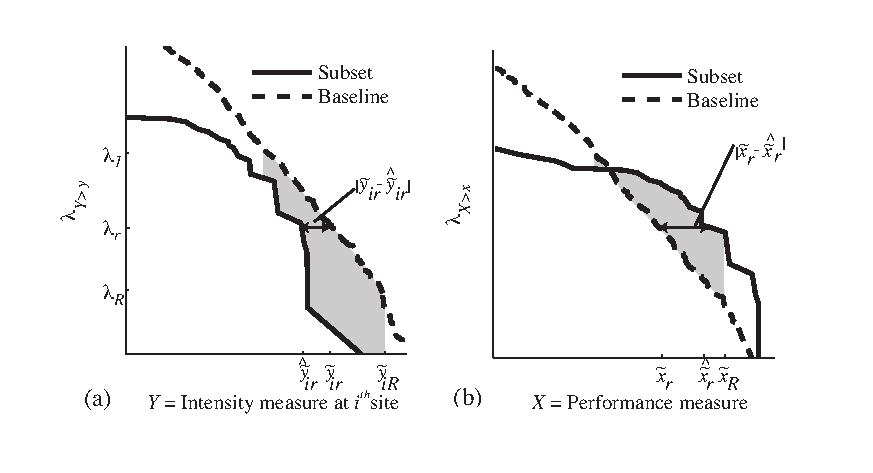
\includegraphics[width=5.6in]{../FIGS/subsets_yr4.eps} %VORSICHT: this is a hack. It should be 5.6 inches wide but somehow by importing it and saving it from Illustrator it shrunk so I had to reduce the width to keep the font size looking reasonable.
%\subfigure[Performance measure]{\includegraphics[width=2.8in]{../FIGS/yr.jpg}\label{fig:yr}} 
\caption{Relationship of error between the subset and the extensively-sampled baseline set of maps for (a) the empirical ground-motion intensity exceedance curves, and (b) the empirical performance measure exceedance curves. The solid line represents an example subset of maps chosen by optimization and the dotted line represents an extensively-sampled baseline set of maps. The grey-colored regions are related to the error and show where the curves differ; the optimization objective function minimizes the sum of the vertical distances between the curves.}
\label{fig:yirs}
\end{figure}

We now aim to choose a set of $k$ damage maps and corresponding ground-motion intensity maps, each with a corresponding adjusted annual rate of occurrence $w_{j'}$, from a set of $J$ candidate maps that provides a good representation of the earthquake hazard and performance risk. In other words, we want to approximate the profile of the loss exceedance curves of the ground-motion shaking intensity and performance measures. We do this by choosing a subset of damage maps and corresponding ground-motion intensity maps that minimizes the differences between the loss exceedance curves of an extensively-sampled baseline set and resulting subset over a range of return periods of interest. This region corresponds to error (shaded in  Figure~\ref{fig:yirs}). This can be expressed as:
%

%
\begin{subequations}
\label{eq:optim}
\begin{align}
\text{minimize} \notag \\
        & \alpha \| \diag{\boldsymbol\lambda}^{-1} (\boldsymbol\lambda - \Psi \textbf{w}) \|_1  + (1-  \alpha) \sum_{i=1}^{\nu} \| \diag{\boldsymbol\lambda}^{-1} (\boldsymbol\lambda - \Theta_i \textbf{w}) \|_1 \label{eq:objfunc} \\
    \text{subject to} \notag \\
        & \textbf{Card}(\textbf{w}) \leq k, \label{eq:const1}\\
        & \textbf{0} \leq \textbf{w}, \label{eq:const2} 
\end{align}
\end{subequations}
with variable $\textbf{w} \in \mathbb{R}^{J \times 1}$. Here each element of $\textbf{w}$, $w_{j'}$, represents the adjusted annual occurrence rate for the $j'^{th}$ damage map and corresponding ground-motion intensity map. The $\textbf{Card}(\textbf{w})$ denotes the cardinality (number of non-zero elements) of the vector $\textbf{w}$. The $\| \|_1$ represent the $L^1$-norm, which is simply the sum of absolute values of the vector. The vector $\textbf{0} \in \mathbb{R}^{J \times 1}$ is the vector of zeros. The vector $\boldsymbol\lambda$ is a vector of constants, $\lambda_1, \ldots, \lambda_R$; the elements of this vector represent the annualized exceedance rates, corresponding to $R$ discretized return period values, where the vector element corresponding to the $r^{th}$ return period equals $\frac{1}{\lambda_r}$.  The matrix $\diag{\boldsymbol\lambda}^{-1}$ is a matrix with all zeros except on the diagonals. 
Also, $\Psi  \in \mathbb{R}^{R \times J} $ is a matrix of constants, 
where for each entry of the matrix, $\psi_{r, j'} = \mathbbm{I}\{ x_{j'} \geq \tilde{x}_r \}$. The constant $\tilde{x}_r$ is the performance measure at the $r^{th}$ return period from an extensively-sampled set of damage maps ($\lambda_r = \lambda_{X \geq \tilde{x}_r}$).
% for return period indices $r  = 1, \ldots, R$. The constant $x_{j'}$ is the performance 
Similarly, $\Theta_i \in \mathbb{R}^{R \times J}$ is a matrix of constants corresponding to the $i^{th}$ site used in the objective function, where for each entry of the matrix, $\theta_{i, r, j'} =  \mathbbm{I}\{ y_{ij'} \geq \tilde{y}_{ir} \}$ for  $i$ denoting the indices of sites at which the objective function will be minimized ($i = 1, \dots, \nu$, where $\nu$ is less than or equal to $n$, the total number of sites of interest). The constant $\tilde{y}_{ir}$ is the ground-motion intensity value at the $r^{th}$ return period from an extensively-sampled set of ground-motion intensity maps (i.e., $\lambda_r = \lambda_{Y \geq \tilde{y}_{ir}}$).
Furthermore, the factor $\alpha$ in the objective function controls the contribution from the ground-motion intensity versus the performance measure. 

The objective function \eqref{eq:objfunc} minimizes the gaps between the exceedance rate curves from the baseline set and from the subset; each site considered in the objective function contributes a ground-motion intensity exceedance rate curve and the whole system also contributes one performance measure exceedance rate curve. Multiplying these values by $\diag{\boldsymbol\lambda}^{-1}$ in the objective function forces lower errors at larger return periods, typically of greatest engineering interest. The second term of the objective function  \eqref{eq:objfunc}, which sums up values related to the ground-motion intensity over all sites, corresponds to the objective function and definition of the error, as expressed as a constraint, in~\cite{han_probabilistic_2012}.
However, our new formulation includes an additional term related to the relatively computationally-cheap proxy performance measure (first term of  \eqref{eq:objfunc}). It also introduces the contribution factor $\alpha$. 
%Han and Davidson's mixed-integer optimization problem for selecting ground-motion intensity maps \cite{han_probabilistic_2012}; we introduce additional constraints to minimize the error in estimating the exceedance curve of a relatively computationally-cheap proxy performance measure,  describe the corresponding new variables, and simplify the expression for clarity. 
%Furthermore, we have reduced the number of variables by including the difference between the curves directly in the objective function; this reduction of variables can reduce computational effort. 
It also differs from most recent work in \cite{gearhart_optimization-based_2014}, because although the objective function in that work also contains a contribution factor and two terms, it considers marginal distributions of bridge damage state and the covariance in the bridge damage between pairs of bridges.  That work is limited to a single ground-motion intensity scenario; that optimization formulation does not explicitly consider consistency with the input distributions of the ground-motion intensity or network performance. This work, in contrast, considers uncertainty in the ground motion maps and uses a proxy network-wide performance in the objective function. We have also introduced a condensed form of the objective function and constraints, as compared to the more verbose mixed-boolean form in these other papers.

The first constraint  \eqref{eq:const1} specifies that the number of maps in the subset equals $k$. The second constraint \eqref{eq:const2} limits the value of each $w_{j'}$ to be non-negative, which is consistent with the physical interpretation of annual occurrence rates. 

%Because one of the constraints specifies that some of the variables must be binary integers, this is an example of a mixed-integer programming problem. 
Since the objective function and the second constraint are linear functions of the variables and constants---but there is a constraint on the cardinality of the set---this is an example of a convex problem with a cardinality constraint, which is nonconvex and NP-hard~\cite{boyd_l1-norm_2014}. %http://www.stanford.edu/class/ee364b/lectures/l1_slides.pdf
One general approach for solving this type of problem is branch-and-bound methods, which find a global solution to nonconvex problems by calculating upper and lower bounds on the optimal value for smaller and smaller parts of the domain of the random variables~\cite{lawler_branch-and-bound_1966,balakrishnan_branch_1991}. They maintain a provable upper and lower bound on the optimal value. While in the worst case the computational time grows exponentially with the number of random variables, in practice, the problem can require less computational effort~\cite{boyd_convex_2004}. The problem can also be solved through heuristics, as we will now discuss.

\subsection{Alternative ground-motion intensity map selection: relaxed problem with convex constraints}
\label{sec:alternativeSelect}
%The original problem~\eqref{eq:optim} has nonconvex constraints, $\textbf{Card}(\textbf{w}) \leq k$. 
To solve this problem more efficiently, we consider a convex relaxation of the map selection problem by replacing the nonconvex cardinality constraint~\eqref{eq:const1} with the convex constraints that  the sum of the $w_{j'}$ is less than or equal to $w_{tot}$, where the constant $w_{tot}$ is the sum of the original annual occurrence rates of all $J$ input maps. In other words, 
\begin{subequations}
\label{eq:optimb}
\begin{align}
\text{minimize} \notag \\
        & \alpha \| \diag{\boldsymbol\lambda}^{-1} (\boldsymbol\lambda - \Psi \textbf{w}) \|_1  + (1-  \alpha) \sum_{i=1}^{\nu} \| \diag{\boldsymbol\lambda}^{-1} (\boldsymbol\lambda - \Theta_i \textbf{w}) \|_1 \label{eq:objfuncb} \\
    \text{subject to} \notag \\
        & \| \textbf{w} \|_1 \leq w_{tot}, \label{eq:const1b}\\
        & 0 \leq \textbf{w}, \label{eq:const2b} 
\end{align}
\end{subequations}
where the parameters and variables are defined above.

This problem is now a convex optimization, because the objective function and the new constraint on $\textbf{w}$ are linear; it is an example of linear programming. One possible method for solving this  basic linear programming problem is an interior point solver~\cite{udell_bounding_2014,boyd_convex_2004}. An optimal value is guaranteed to exist~\cite{boyd_convex_2004}. Furthermore, the value of the objective function using these relaxed constraints provides a lower bound on the optimal value of the original formulation~\eqref{eq:objfunc}~\cite{boyd_convex_2004}. For testing the quality of the results, an upper bound on the original formulation~\eqref{eq:objfunc} could be found by a feasible solution; readers are referred to~\cite{udell_maximizing_2013,boyd_convex_2004} for more details.%section 3.1.5 of  S. Boyd and L. Vandenberghe, Convex Optimization. Cambridge,
%U.K.: Cambridge Univ. Press, 2004.

However, the solution to this problem is different from the original formulation~\eqref{eq:objfunc}, because there could be more than $k$ non-zero values. We adopt the heuristic method from Joshi and Boyd \cite{joshi_sensor_2009} to use the solution of the relaxed problem to select a subset. The maps with the $k$ largest weights are selected and then renormalized so that the sum of the $k$ new occurrence rates equals the cumulative annual rate of the input set of maps, $ w_{tot}$.  Upon implementation, the results are reasonably consistent with the baseline set and the errors using the original formulation. However, when the cardinality of the subset is very small, the chosen set of maps and corresponding annual occurrence rates tend to correspond to high error. We illustrate both trends in Section~\ref{sec:case}. Readers may also consider replacing $w_{tot}$ with a generic parameter and adjusting its value to force the number of non-zero $w_{j'}$ values to be less than $k$; the map selection problem here has parallels to the sparse signal reconstruction problem in Electrical Engineering~\cite{boyd_l1-norm_2014}. %slides 18-19 and 26-28 of http://www.stanford.edu/class/ee364b/lectures/l1_slides.pdf



%Since an
%SOCP problem is a convex optimization problem, a global solution of a mixed-integer second-order
%cone programming problem can be found by using, e.g., a branch-and-bound method; see, e.g.,
%Atamt�urk and Narayanan [4], Drewes and Pokutt [6] and Vielma et al. [32] for more account. This
%guaranteed global optimality is a major advantage of the proposed approach to the existing local
%and/or heuristic algorithms for design of damper distribution.
%
%make it more computationally feasible than the original formulation (eq.~\ref{eq:original}). However, it has the problem that it tends to produce results with a higher error at a very low desired number of maps, $k$, in the authors' experience. This will be illustrated in the case study below.

\subsection{Evaluation of error in the selected subset} \label{sec:errors}
We now evaluate the error in the estimation of exceedance rates between the selected subset of ground-motion intensity maps and the baseline set. A simple approach is to compute the value of the relevant term of the objective function of the optimization formulation. Alternatively, Han and Davidson \cite{han_probabilistic_2012} defined a Mean Hazard Curve Error (MHCE) for the ground-motion intensity as follows:
\begin{equation}
MHCE = \frac{1}{n R} \sum_{r=1}^R \sum_{i=1}^n \left| \frac{\tilde{y}_{ir} - \hat{\tilde{y}}_{ir}}{\tilde{y}_{ir}} \right|,
\label{eq:MHCE}
\end{equation}
where $\hat{\tilde{y}}_{ir}$ is the estimated ground-motion intensity using the selected subset of maps for the $r^{th}$ return period and $i^{th}$ site and the other variables have been defined above. This equation sums the normalized differences in the ground-motion intensity estimated from the subset and the baseline set over sites and return periods (Figure~\ref{fig:yirs}{\color{red}(a)}). 

We extend this error metric to evaluate the error in performance measure exceedance curves between the subset and the baseline set. This Mean Performance Measure Curve Error (MPMCE) is defined as 
\begin{equation}
MPMCE = \frac{1}{R} \sum_{r=1}^R \left| \frac{\tilde{x}_{r} - \hat{\tilde{x}}_{r}   }{\tilde{x}_{r}} \right|,
\label{eq:MPMCE}
\end{equation}
where $\hat{\tilde{x}}_{r}$ is the estimated performance measure value using the selected subset of maps for the $r^{th}$ return period and the other variables have been defined above (Figure~\ref{fig:yirs}{\color{red}(b)}). 

